\chapter{Implementation}
\label{chapter:implementation}

GatePlay is implemented in the HTML/CSS/JavaScript stack. A brief overview of what HTML, CSS, and JavaScript are is provided in section~\ref{chapter:background}. This chapter will go through the main JavaScript files in the project and the relationships between them.

Some of the JavaScript files are not my own work, but open-source libraries. Re-using others' code lets me focus on implementing the parts unique to GatePlay and avoid writing boilerplate code\footnote{http://en.wikipedia.org/wiki/Boilerplate\_code}. The most important libraries are described throughout this chapter.

The implementation is split in to two main, independent parts: the workbench (described in section~\ref{section:workbench}) and the simulator (described in section~\ref{section:simulator}). I explain how  I linked the parts together in section~\ref{section:application}.

\section{Getting Started}
GatePlay is made up of many JavaScript files, but when its URL is visited the only file downloaded is the main HTML file: \textit{index.html}. The index must then direct the user's browser to download the additional files needed to run GatePlay.

JavaScript files are loaded into the browser using HTML Script tags, in the order the Script tags appear in the document. JavaScript scripts may use methods or variables defined in other scripts provided that those scripts have already been loaded and run in advance.

That means that if $model.js$ and $view.js$ are JavaScript scripts, and $view.js$ depends on $model.js$, then $model.js$'s Script tag must appear first or the website will fail to load. An example is shown in figure~\ref{fig:scripttags}.

\begin{figure}[H]
\begin{lstlisting}[language=html]
<!-- componentview depends on component -->
<!-- Therefore we ensure component is loaded first -->
<script type="text/javascript" src=".../component.js"></script>
<script type="text/javascript" src=".../componentview.js"></script>
\end{lstlisting}
\caption{Example use of Script tags}
\label{fig:scripttags}
\end{figure}

\subsection{Require.js}
It is time consuming for a human to find and type out a correct ordering for the Script tags, and it would need to be updated every time a file is added or removed, or sometimes if a file were modified.

Require.js is a JavaScript file loader which automatically loads files in a correct order. Each JavaScript file declares its direct dependencies, and Require.js will ensure they are all loaded correctly when the website loads.

Every JavaScript file it GatePlay is configured to work with Require.js, but code listings after this point will omit the Require.js machinery for the sake of clarity.

\begin{figure}[H]
\begin{lstlisting}[language=JavaScript]
// componentview.js

require([
	// Declare the path of each file we require	
	"canvas/model/component"
], function(Component) {
	// Each included file is run, and we can give a name to whatever it returns if desired
	var myComponent = new Component();
	...
});
\end{lstlisting}
\caption{An example file which uses Require.js}
\end{figure}

\section{The Workbench}
\label{section:workbench}
GatePlay's workbench is where we create and view circuits. I used the model-view-controller\footnote{http://en.wikipedia.org/wiki/Model-view-controller} design pattern to simply development. MVC programs are split in to three types of component:

\begin{itemize}
	\item \textbf{Models} which store some part of the state of the application
	\item \textbf{Views} which display a representation of one of the models to the user
	\item \textbf{Controllers} which process user input and updates the appropriate models
\end{itemize}

The interactions between the components can be seen in figure~\ref{fig:mvc}. By separating out the concerns of the program it becomes possible to, for example, add new views for your models without needing to change the models or controllers themselves.

\begin{figure}[H]
	\centering
	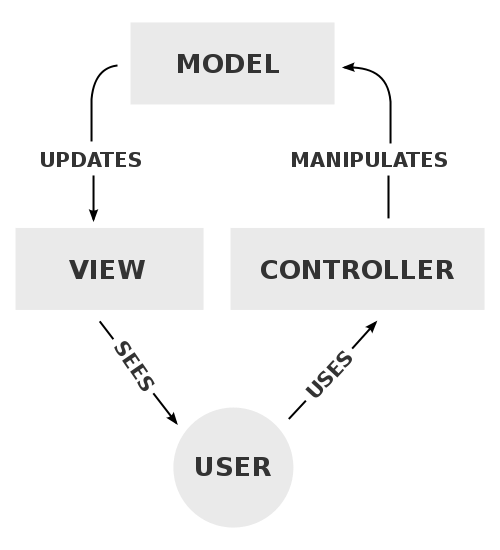
\includegraphics[width=0.5\textwidth]{mvc.png}
	\caption{Interaction of MVC Components, from Wikipedia\cite{Wikipedia: MVC Image}}
	\label{fig:mvc}
\end{figure}

\subsection{MVC with Backbone.js}
Backbone.js\footnote{http://backbonejs.org} is a JavaScript library used to reduce the amount of boilerplate code in developing MVC JavaScript applications by providing predefined notions of models, views, and controllers. A specific example is that Backbone models automatically fire events when any of their fields change value, so I did not have to reimplement that myself.

\subsection{Models}
I first created the models behind the workbench. The top-level model is a \textit{Circuit} model which contains a set of \textit{Component} models and a set of \textit{Wire} models.

Part of the Component model definition is shown in figure~\ref{fig:componentmodel}. The actual model contains some additional helper methods, but they do not add any new state to the model and are not shown. Each Component is given a unique identifier (id), an (x, y) position on the workbench, a width, and input and output counts. The \textit{isValid} flag is set to False if this component is ever over another component (which the Circuit disallows) so it can be drawn in a different colour. \textit{activeInputIndex} and \textit{activeOutputIndex} are set when the user hovers their mouse over an input or an output port, so they may be highlighted in a different colour.

Notice that the height of a Component is a function of its input and output counts.

\begin{figure}
\begin{lstlisting}[language=JavaScript]
var Component = Backbone.Model.extend({
	defaults: function() {
    	return {
        	id: nextId++,
            x: 0,
            y: 0,
            width: 7,
            inputCount: 2,
            outputCount: 1,
            isValid: true,
            activeInputIndex: -1,
            activeOutputIndex: -1
        }
    },

    getHeight: function() {
        return Math.max(this.get("inputCount"), this.get("outputCount")) * 2 + 1;
    }
});
\end{lstlisting}
\caption{Definition of a Component model}
\label{fig:componentmodel}
\end{figure}

Next I created the Wire model (figure~\ref{fig:wiremodel}). The Wire model is very close to the definition of a wire we used in the simulator, except we additionally store a list of \textit{fixed points}. Fixed points are points through which the wire passes on its way from the source component to the target component. Wire segments must be aligned with the x- or y-axis, and the model checks this condition when it is initialised or whenever the fixed points change.

\begin{figure}
\begin{lstlisting}[language=JavaScript]
var Wire = Backbone.Model.extend({
	defaults: function() {
    	return {
        	id: nextWireId++,
        	sourceId: -1,
        	sourcePort: -1,
       	 	targetId: -1,
        	targetPort: -1,
        	fixedPoints: [],
        	truthValue: TruthValue.UNKNOWN
    	}
	},
})
\end{lstlisting}
\caption{Definition of a Wire model}
\label{fig:wiremodel}
\end{figure}

With the Component and Wire models we can create a Circuit model. I will not include the Circuit model code listing as it is long yet simple, but rather describe how it works below. 

As in the simulator, a Circuit on the workbench contains a set of Components and a Set of Wires. The workbench Circuit also has a given width and height which all components and wires must be contained within.

In GatePlay components are not permitted to overlap each other, and it is the Circuit model's responsibility to enforce this. Recall that the Circuit has a given width and height, and each component has a position, width, and height. The Circuit maintains a 2D array where each cell is a point on the workbench, containing the identifier of the component at that position (or an empty flag if no component). When adding a component to the circuit, it calculates the points the new component will occupy and then checks that no component already occupies those cells. If the check fails, then the component will not be added to the model.

\subsection{Views}
Now that we have the back end models for the workbench, it is a matter of displaying them to the user.

To display circuits we need an element on the web page to draw graphics. I used an HTML Canvas element --- a blank slate on which we can draw shapes and images --- as it provides the exact functionality required.

The CircuitView will initialise the canvas, and then delegate to a collection of ComponentViews and WireViews to draw the Components and Wires respectively.

\subsubsection{Fabric.js}
From the user's perspective the workbench is going to contain a collection of objects (components), each of which can be selected and moved. An HTML Canvas is essentially a flat array of pixels and does have any concept of objects on the canvas.

Fabric.js is an canvas framework which wraps HTML Canvas elements with an object model, allowing GatePlay to interact at the level of objects being added to, modified on, and removed from the canvas.

As an example, consider the user moving a component from one position on the workbench to another. With an HTML Canvas I would need to re-calculate and re-draw the background over the component, and then re-draw the component at its new location. Fabric.js already implements this feature, and it is a simple library call to move the component to a new location. Using Fabric.js greatly reduces the amount of code needed to interact with canvases.

Initially GatePlay used a different canvas framework called KineticJS, but due to difficulties getting features like snap-to-grid working I switched to Fabric.js early on in development.

\subsubsection{ComponentView}
An instance of the ComponentView class is responsible for drawing a single instance of a Component model. On instantiation, a ComponentView is passed the canvas it is to draw on and the model it is to draw. The code of the ComponentView is long and simple. Figure~\ref{fig:componentview} contains a reduced version of the code, and I will explain the meaning of each method below. The \textit{this.model.on} calls in the \textit{initialize} method are examples of Backbone.js reducing boilerplate code: when the model is changed the view will update automatically.

\begin{itemize}
	\item The \textbf{render} method draws the component on the canvas. It requests a template for the component's type from a repository of templates (there is a template for $AND$ gates, and $NOT$ gates, and so on) and adds it to the canvas. It also draws the nodes for the input and output ports
	\item The \textbf{setFillColor} method is called when the model's truth value changes. For example $Toggle$s are coloured with the value of their current output, and this method is called when their value changes
	\item The \textbf{activeInputChanged} and \textbf{activeOutputChanged} methods are called when the user hovers over an input or output port respectively. It highlights the hovered port with a different colour so users know that clicking on it will perform an action (starting to draw wires)
\end{itemize}

\begin{figure}
\begin{lstlisting}[language=JavaScript]
Backbone.View.extend({
    initialize: function(options) {
        this.options = options.options;
        this.model = options.model;
        this._template = null;
        this._activePort = null;
		
		// When the model changes, update the view
        this.model.on("change:isValid", this._setFillColor, this);
        this.model.on("change:activeInputIndex", this._activeInputChanged, this);
        this.model.on("change:activeOutputIndex", this._activeOutputChanged, this);
        this.model.on("change:truthValue", this._setFillColor, this);
    },

    render : function() {
        // Render the gate on the canvas
    },

    _setFillColor: function() {
        // Set the fill colour of the component
        // LED's are filled the the colour of their input, for example
    },

    _activeInputChanged: function() {
        // The user is hovering over an input port, so colour it red
    },

    _activeOutputChanged: function() {
        // The user is hovering over an output port, so colour it red
    },
});
\end{lstlisting}
\caption{Definition of a ComponentView}
\label{fig:componentview}
\end{figure}

\subsubsection{WireView}
An instance of the WireView class draws a single Wire model on the canvas. It is very similar to the ComponentView class in that it has a \textit{render} method and a \textit{setWireColor} method (which is called when the wire value changes). The render function draws each segment between fixed points as a straight line and combines them to create one Fabric.js object which is added to the canvas.

\subsubsection{CircuitView}
The CircuitView draws the entire circuit. Its \textit{render} method is shown in figure~\ref{fig:circuitrender}. When the Circuit is rendered, it simply clears the old canvas, and then redraws the components and wires. The SetViews seen in the code listing simply take a set of models and create a view for each model in turn.

\begin{figure}
\begin{lstlisting}[language=JavaScript]
render: function() {
	// Clear old canvas
    this.options.canvas.clear();

    // Draw the components on the grid
    var componentSetView = new ComponentSetView(this.options);
    componentSetView.render();

    // Draw the wires on the grid
    var wireSetView = new WireSetView(this.options);
    wireSetView.render();
},
\end{lstlisting}
\caption{CircuitView render method}
\label{fig:circuitrender}
\end{figure}

\subsection{Controllers}
There is one controller for GatePlay's workbench, simply called \textit{CircuitController}. It handles all the mouse events which occur on the workbench: mouse movement, mouse clicks, hovering over components, and creating box selections.

In fact it delegates all the handling to its event handler. When the user is editing a circuit it is an instance of EditingEventHandler, when running a simulation it is an instance of RunningEventHandler.

\subsubsection{EditingEventHandler}
The EditingEventHandler is by far the biggest class in GatePlay and so does not have a code listing. I will briefly describe how it performs each of its responsibilities:

\begin{itemize}
	\item \textbf{Moving components:} If the user's mouse was clicked over an object (not on an output port), held down, and moved then that object is being dragged. The handler updates the position of the component model in real time
	
	\item \textbf{Drawing wires:} If the user's mouse was clicked over one of an object's output ports, then the user is drawing a wire. Single clicks create a fixed point for the wire, and double clicking cancels drawing. If the user clicks on an empty input port, the appropriate wire is created and added to the model
	
	\item \textbf{Components selected:} GatePlay allows users to drag components over other components temporarily (colouring them red to show it is an invalid position). The component being moved should always appear on top. To implement this, when components are selected they are immediately brought to the front of the canvas 
\end{itemize}

\subsubsection{RunningEventHandler}
When running a simulation should not be possible to move components or draw wires. The only event the RunningEventHandler looks for is the user clicking on a $Toggle$ component. When this happens, the Component model for that $Toggle$ is updated with the new truth value and the simulator is notified of the change.

\section{The Simulator}
\label{section:simulator}
The implementation of GatePlay's simulator is a relatively straightforward implementation of the algorithms and ideas explained in chapter~\ref{chapter:simulation}. The following six classes fully implement the simulator:

\begin{itemize}
	\item \textbf{truthvalue.js} defines constants $True$, $False$, and $Unknown$
	\item \textbf{component.js} defines a Component by its input count, output count, and evaluation function
	\item \textbf{wire.js} defines a Wire by its input component and port, output component and port, and truth value
	\item \textbf{circuitevent.js} defines a CircuitEvent by component, port, timestamp, and value
	\item \textbf{functions.js} contains definitions of all the Evaluation Functions available to the simulator 
	\item \textbf{circuit.js} is the only class which need be visible from outside the simulator. It has an interface to add components and wires. Circuit.js implements the algorithm for the event loop. 
\end{itemize}

\subsection{Blinker Events}
Recall section~\ref{subsec:initial} that $Blinker$ components toggle their output value at a set interval. Each $Blinker$ has its own, potentially unique, interval.

To implement this, a $Blinker$ component's evaluation function (shown in figure~\ref{fig:blinkereval} determines it truth value based on the simulation clock. Since $Blinker$s have no inputs they will never be processed by the event loop, so we need to handle $Blinker$s differently.

\begin{figure}
\begin{lstlisting}[language=JavaScript]
Blinker.prototype._doEvaluate = function(argList, clock) {
    var era = Math.floor(clock / this._interval);
    var parity = era % 2;
    if (parity === 0) {
        return [TruthValue.TRUE];
    } else {
        return [TruthValue.FALSE];
    }
};
\end{lstlisting}
\caption{Implementation of $Blinker$'s evaluation function}
\label{fig:blinkereval}
\end{figure}

The solution implemented in GatePlay is to add a new circuit event for every $Blinker$, \textit{every} clock tick. For a $Blinker$ with interval $2$, we would add $True$ events at simulated time $0$ and $1$, $False$ events at simulated time $2$ and $3$, and so on. We rely on culling to eliminate the unnecessary events.

The algorithm described above if very easy to implement, but clearly inefficient if there were a large number of $Blinker$s. A better algorithm where we only add one circuit event per $Blinker$ per interval is outlined in figure~\ref{fig:blinkerqueue}. We store in a priority queue the next event for each $Blinker$. Whenever we pop an event from the queue we replace it with an event for the next time the corresponding blinker will change value.

Note that the \textit{blinkerEventQueue} is just a subset of the main event queue, and we could actually merge this code with the event loop. However doing so would couple our implementation of the general event queue with that of a specific type of component and not be good software engineering practice.

\begin{figure}
\begin{lstlisting}[language=JavaScript]
function tick() {
	// For each blinker event which is happening at this time
	while (this._blinkerEventQueue.peek().time <= this._clock) {
		var event = this._blinkerEventQueue.pop();
		this._addEvent(event);
		
		var blinker = this.getComponent(event.sourceId);
		var nextTime = event.eventTime + blinker.get("interval");
		var nextValue = blinker.evaluate([], nextTime);
		var nextEvent = new CircuitEvent(nextTime, event.sourceId, event.sourcePort, nextValue);
		this._blinkerEventQueue.add(nextEvent);
	}
	
	// Event loop goes here
}
\end{lstlisting}
\caption{}
\label{fig:blinkerqueue}
\end{figure}

\section{Drag-and-drop}
One of the requirements of GatePlay was that it be easy to use, and being able to drag-and-drop components from the left-bar is important in satisfying that requirement. Implementing drag-and-drop is can be split in to three main sub problems:

\begin{enumerate}
	\item Drawing the components in the left-bar
	\item Allow dragging components from the left side-bar
	\item Adding components to the workbench where they dropped
\end{enumerate}

To draw the components on the left-bar I create an HTML Image element for each type of component. When the page loads, GatePlay creates an image of each type of Component and displays the image in one of the Image elements. Creating images for each component is handled by the \textit{createThumbnail} function: \textit{createThumbnail} creates a temporary canvas for each component and renders the component on it. This canvas can be converted to an image file by a Fabric.js library call.

Dragging and dropping is an interaction supported by the jQueryUI\footnote{http://http://jqueryui.com/} library, which GatePlay uses. The components in the left-bar are marked as \textit{Draggable} and the main workbench is marked as \textit{Droppable}. With a small amount of configuration, components can be dragged from the left-bar on to the workbench.

Adding the components to the workbench is done by handling jQueryUI's \textit{drop} event which is called when components are dropped on the workbench. The handler converts the location from global co-ordinates (number of pixels from the top-left hand corner of the browser window) to workbench co-ordinates (number of grid cells from the top-left hand corner of the workbench), and instructs the workbench to add a new component there. This is done by the Application class described in the next section.

\section{Tying GatePlay Together}
\label{section:application}
The implementation discussed so far has multiple distinct parts which have no knowledge of each other: the workbench, the simulator, and droppable interactions. We create a new class \textit{Application} which ties the pieces together as shown in figure~\ref{fig:application}

\begin{figure}[H]
    \centering
    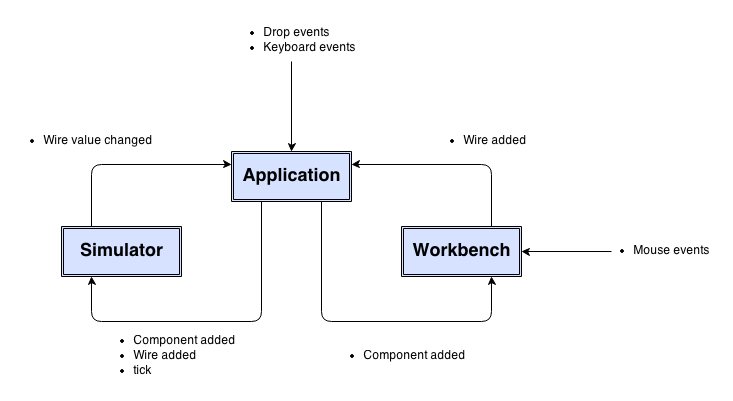
\includegraphics[width=\textwidth]{application.png}
    \caption{Information flow in GatePlay}
    \label{fig:application}
\end{figure}

The Application is the first part of GatePlay's code to be executed, and creates the workbench Circuit model and CircuitView view when it is initialised. It is Application which handles jQueryUI's \textit{drop} event, listens for presses of the Delete key, and notifies the workbench when the mode change to Editing or Running.

When the user clicks to start simulating their circuit, Application copies across all the circuit information from the workbench into a new simulator object (the code listing is shown in figure~\ref{fig:nowrunning}). It also registers an event handler with the simulator to update the value of the wires on the workbench when they change in the simulator.

By making GatePlay modular in this way, it is very easy to change one part of the code without changing the rest of it.

\begin{figure}
\begin{lstlisting}
ApplicationState.prototype._nowRunning = function() {
    this._setClock(0);

    // Create new simulator
    var simulation = new SimCircuit();
    this._simulation = simulation;

    // Add components
    var components = this._canvasModel.get("components");
    _.each(components.models, function(c) {
        simulation.addComponent(c.get("id"), c.get("templateId"), c.get("inputCount"), c.get("outputCount"), c.get("cArg"));

        if (c.get("templateId") === "toggle" || c.get("templateId") === "blinker") {
            c.set("truthValue", "True");
        } else if (c.get("templateId") === "led") {
            c.set("truthValue", "Unknown");
        }
    })

    // Add wires
    var wires = this._canvasModel.get("wires");
    _.each(wires.models, function(wire) {
        simulation.addWire(wire.get("id"), wire.get("sourceId"), wire.get("sourcePort"), wire.get("targetId"), wire.get("targetPort"));

        wire.set("truthValue", "Unknown");
    })

    simulation.initialize();
    simulation.addWireEventListener(function(id, truthValue) {
        var wire = wires.get(id);
        wire.set("truthValue", truthValue);

        var source = components.get(wire.get("sourceId"));
        if (source.get("templateId") === "toggle" || source.get("templateId") === "blinker") {
            source.set("truthValue", truthValue);
        }

        var target = components.get(wire.get("targetId"));
        if (target.get("templateId") === "led") {
            target.set("truthValue", truthValue);
        }
    })
};
\end{lstlisting}
\caption{Application.js's nowRunning method}
\label{fig:nowrunning}
\end{figure}